\documentclass{article}
\usepackage{tikz}
\usetikzlibrary{arrows.meta}
\usetikzlibrary{calc}
\usepackage{mathtools}
\usepackage{amsmath}
\usepackage{amssymb}
\usepackage{amsfonts}
\usepackage{graphicx}
\usepackage{float}
\usepackage{multirow}
\usepackage{verbatim} \usepackage{listings}

\linespread{1.3}
\setlength{\parindent}{0em}
\setlength{\parskip}{1em}
\setcounter{secnumdepth}{0}
\setcounter{MaxMatrixCols}{20}
\renewcommand{\arraystretch}{1.5}

\newcommand{\ts}{\textsuperscript}
\newcommand{\diff}{\mathop{}\!\mathrm{d}}
\newcommand{\prob}{\mathbb{P}}
\newcommand{\expect}{\mathbb{E}}
\newcommand{\var}{\text{Var}}

\DeclarePairedDelimiter{\abs}{\lvert}{\rvert}
\DeclarePairedDelimiter\norm{\lVert}{\rVert}
\DeclarePairedDelimiter\p{\lparan}{\rparan}

\title{STAT3004 Assignment 3}
\author{Joshua Hwang (44302650)}

\begin{document}
\section{1}
\subsection{a}
By drawing the Markov chain we reveal our possible transitions.

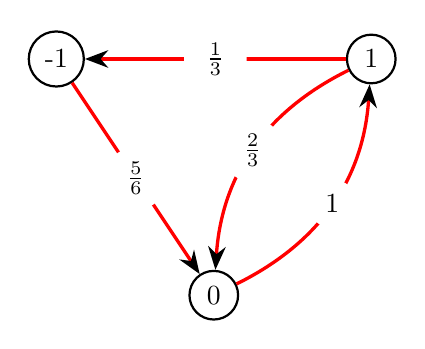
\begin{tikzpicture}
    \begin{scope} [every node/.style={circle,thick,draw}]
        \node (-1) at (0,0) {-1};
        \node (0) at (2,-3) {0};
        \node (1) at (4,0) {1};
    \end{scope}

    \begin{scope}[>={Stealth[black]},
            every node/.style={fill=white,circle},
            every edge/.style={draw=red,very thick}]
        \path [->] (-1) edge node {$\frac{5}{6}$} (0);
        \path [->] (1) edge node {$\frac{1}{3}$} (-1);
        \path [->] (0) edge[bend right=30] node {$1$} (1);
        \path [->] (1) edge[bend right=30] node {$\frac{2}{3}$} (0);
    \end{scope}
\end{tikzpicture}

We note that if $X_0 = 0$ then there is no way to get $X_2 = 1$ thus \\
$\prob(X_2 = 1 | X_0 = 0) = 0$.

We now use this same technique to determine $\prob(X_2 = 1)$,
\begin{align*}
    \prob(X_2 = 1) &= \prob(X_2 = 1 | X_0 = 0) \prob(X_0 = 0) \\
                   &+ \prob(X_2 = 1 | X_0 = 1) \prob(X_0 = 1) \\
                   &+ \prob(X_2 = 1 | X_0 = -1) \prob(X_0 = -1) \\
    \prob(X_2 = 1) &= 0 \times \prob(X_0 = 0) \\
                   &+ \frac{2}{3} \prob(X_0 = 1) \\
                   &+ \frac{5}{6} \prob(X_0 = -1) \\
    \prob(X_2 = 1) &= \frac{2}{3} \times \frac{1}{2}
                    + \frac{5}{6} \times \frac{1}{6} \\
    \prob(X_2 = 1) &= \frac{1}{3} + \frac{5}{36} \\
    \prob(X_2 = 1) &= \frac{17}{36} \\
\end{align*}

\subsection{b}
To get the expectation we need to repeat this process for $\prob(X_2 = -1)$
and $\prob(X_2 = 0)$.
\begin{align*}
    \prob(X_2 = -1) &= \prob(X_2 = -1 | X_0 = 0) \prob(X_0 = 0) \\
                    &+ \prob(X_2 = -1 | X_0 = 1) \prob(X_0 = 1) \\
                    &+ \prob(X_2 = -1 | X_0 = -1) \prob(X_0 = -1) \\
    \prob(X_2 = -1) &= \frac{1}{3} \prob(X_0 = 0) \\
                    &+ \frac{1}{3} \times \prob{1}{6} \prob(X_0 = 1) \\
                    &+ \frac{1}{6} \times \frac{1}{6} \prob(X_0 = -1) \\
    \prob(X_2 = -1) &= \frac{1}{3} \times \frac{1}{3} \\
                    &+ \frac{1}{18} \times \frac{1}{2} \\
                    &+ \frac{1}{36} \times \frac{1}{6} \\
    \prob(X_2 = -1) &= \frac{31}{216}
\end{align*}
\begin{align*}
    \prob(X_2 = 0) &= \prob(X_2 = 0 | X_0 = 0) \prob(X_0 = 0) \\
                   &+ \prob(X_2 = 0 | X_0 = 1) \prob(X_0 = 1) \\
                   &+ \prob(X_2 = 0 | X_0 = -1) \prob(X_0 = -1) \\
    \prob(X_2 = 0) &= \frac{83}{216}
\end{align*}

We can now determine $\expect[X]$ and $\expect[X^2]$.
\begin{align*}
    \expect[X_2]&= 0 \times \prob(X_2 = 0) + \prob(X_2 = 1) - \prob(X_2 = -1) \\
                &= \frac{17}{36} - \frac{31}{216} \\
                &= \frac{71}{216} \\
\end{align*}

\begin{align*}
    \expect[X_2^2] &= 0 \times \prob(X_2 = 0)
                    + \prob(X_2 = 1) + \prob(X_2 = -1) \\
                   &= \frac{17}{36} + \frac{31}{216} \\
                   &= \frac{133}{216} \\
\end{align*}

\begin{align*}
    \var X_2 &= \expect[X_2^2] - \expect{[X_2]}^2 \\
             &= \frac{133}{216} - {(\frac{71}{216})}^2 \\
             &= \frac{23687}{46656} \\
\end{align*}

Thus, $\expect[X_2] = \frac{71}{216}$ and $\var[X_2] = \frac{23687}{46656}$.

\subsection{c}
A stationary distribution is defined as $\pi P = \pi$.
\begin{align*}
    \begin{bmatrix}
        a & b & c \\
    \end{bmatrix}
    \begin{bmatrix}
        \frac{1}{6} & \frac{5}{6} & 0 \\
                  0 &           0 & 1 \\
        \frac{1}{3} & \frac{2}{3} & 0 \\
    \end{bmatrix}
    &=
    \begin{bmatrix}
        a & b & c \\
    \end{bmatrix}
\end{align*}

From this we get four equations.
\begin{align*}
    a + b + c &= 1 \\
    \frac{1}{6} a + \frac{1}{3} c &= a \\
    \frac{5}{6} a + \frac{2}{3} c &= b \\
    b &= c \\
\end{align*}

Solving these equations gives us only a single solution.
\begin{align*}
    a &= \frac{1}{6} \\
    b &= \frac{5}{12} \\
    c &= \frac{5}{12}
\end{align*}

We diagonalise the matrix $P$ so it becomes easier to raise to powers.
From here we take $S \Lambda^n S^{-1}$ with $n \to \infty$. Out of the three
eigenvalues, $\lambda = -\frac{1}{2}, -\frac{1}{3}, 1$,
we find only one of them is $\geq 1$.

\begin{align*}
    P
    &=
    \begin{bmatrix}
        \frac{5}{2} &  5 & 1 \\
                 -2 & -3 & 1 \\
                  1 &  1 & 1 \\
    \end{bmatrix}
    \begin{bmatrix}
        -\frac{1}{2} &            0 & 0 \\
                   0 & -\frac{1}{3} & 0 \\
                   0 &            0 & 1 \\
    \end{bmatrix}
    \begin{bmatrix}
        -\frac{2}{3} & -\frac{2}{3} & \frac{4}{3} \\
         \frac{1}{2} &  \frac{1}{4} & -\frac{3}{4} \\
         \frac{1}{6} & \frac{5}{12} & \frac{5}{12} \\
    \end{bmatrix} \\
    P^n
    &=
    \begin{bmatrix}
        \frac{5}{2} &  5 & 1 \\
                 -2 & -3 & 1 \\
                  1 &  1 & 1 \\
    \end{bmatrix}
    \begin{bmatrix}
        -\frac{1}{2}^n &              0 & 0 \\
                     0 & -\frac{1}{3}^n & 0 \\
                     0 &              0 & 1^n \\
    \end{bmatrix}
    \begin{bmatrix}
        -\frac{2}{3} & -\frac{2}{3} & \frac{4}{3} \\
         \frac{1}{2} &  \frac{1}{4} & -\frac{3}{4} \\
         \frac{1}{6} & \frac{5}{12} & \frac{5}{12} \\
    \end{bmatrix} \\
    P^n
    &=
    \begin{bmatrix}
        \frac{5}{2} &  5 & 1 \\
                 -2 & -3 & 1 \\
                  1 &  1 & 1 \\
    \end{bmatrix}
    \begin{bmatrix}
        0 & 0 & 0 \\
        0 & 0 & 0 \\
        0 & 0 & 1 \\
    \end{bmatrix}
    \begin{bmatrix}
        -\frac{2}{3} & -\frac{2}{3} & \frac{4}{3} \\
         \frac{1}{2} &  \frac{1}{4} & -\frac{3}{4} \\
         \frac{1}{6} & \frac{5}{12} & \frac{5}{12} \\
    \end{bmatrix} \\
    P^n
    &=
    \begin{bmatrix}
        \frac{1}{6} & \frac{5}{12} & \frac{5}{12} \\
        \frac{1}{6} & \frac{5}{12} & \frac{5}{12} \\
        \frac{1}{6} & \frac{5}{12} & \frac{5}{12} \\
    \end{bmatrix}
\end{align*}

Thus our stationary distribution is our limiting distribution.

\subsection{d}
The code used is below.
\lstinputlisting[language=python]{q1d.py}

These are the results.
\begin{verbatim}
==================================================
P(X_2=1) ~ 0.45
standard error = 0.015740004693383852
P(X_2=1) = 0.4722222222222222
--------------------------------------------------
E[X_2] ~ 0.307
standard error = 0.022343908571470908
E[X_2] = 0.3287037037037037
--------------------------------------------------
Var(X_2) ~ 0.49925025025025105
standard error = 0.016619784188529146
Var(X_2) = 0.5076946159122085
==================================================
\end{verbatim}

\section{2}
\subsection{a}
Transience is defined as $r_{xx} < 1$. It should be noted that $x \to y$ means
$r_{xy} > 0$. Also note that $r_{xy} = 1$ means that there exists a
natural number $n$ such that we start at state $x$ and arrive at state $y$ by
$n$ steps.

We attempt to prove by contradiction. Assume $x$ is not transient, $r_{xx} = 1$.

Since we're guaranteed to end up back at state $x$ there must be a guaranteed
way to get from $y$ to $x$ (since there is a non-zero probability we end up at
state $y$ starting from state $x$); $r_{yx} = 1$.
This leads to a contradiction since it was previously stated
that $r_{yx} < 1$. Therefore $x$ is transient, $r_{xx} < 1$.

\subsection{b}
We attempt to prove via contradiction.
If $x$ is transient then $r_{xx} < 1$. We also have $x \leftrightarrow y$.
We suppose that $y$ is not transient, $r_{yy} \nless 1$ thus $r_{yy} = 1$.
As stated in the lectures,
if $x$ is recurrent and $x \to y$ then $y$ is also recurrent and $y \to x$.

Thus we conclude that $x$ is recurrent which is a contradiction of our previous
claim.

Therefore we conclude that $y$ must be transient. Transience is a property
shared by those in the same communicating class.

\subsection{c}
Note that if $\mathcal{C}$ is not closed then $\exists x \in \mathcal{C}$
where $x \to y$ and $y \notin \mathcal{C}$.

We attempt to prove that this state $x$ is transient via contradiction.
Suppose it's recurrent. As stated in the lectures,
if $x$ is recurrent and $x \to y$ then $y$ is also recurrent and $y \to x$.
This means that our state $x$ and state $y$ are part of the same communicating
class. This is a contradiction to our previous point that
$y \notin \mathcal{C}$.

Thus we conclude that state $x$ is transient. Since $x$ is transient and we know
that transience is a class property, $\mathcal{C}$ is a transient communicating
class.

\section{3}
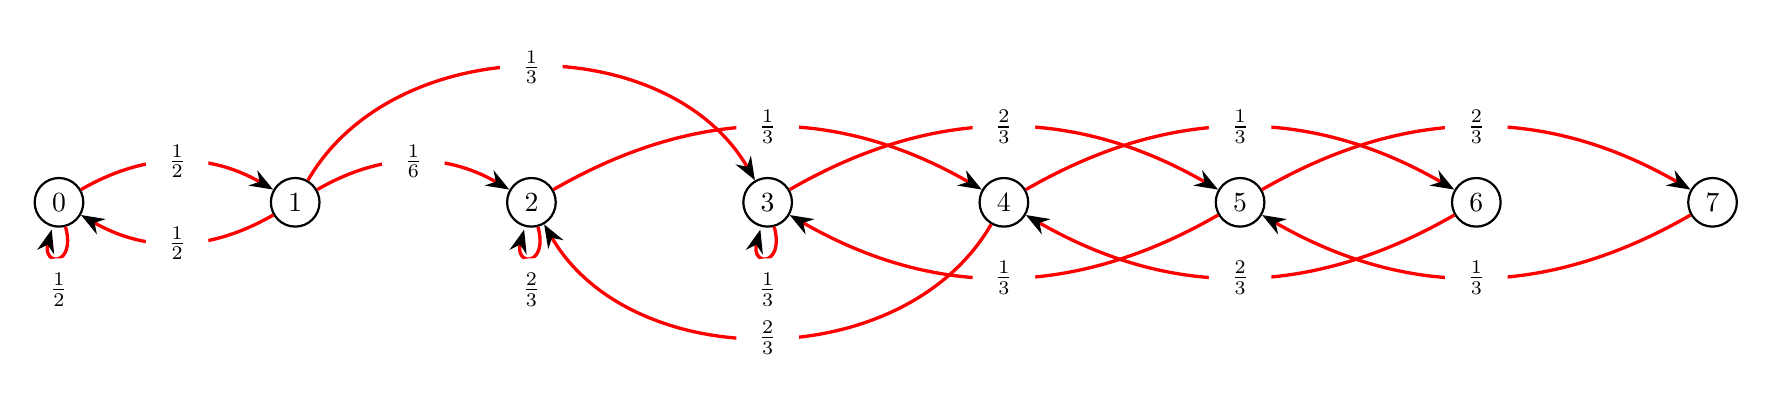
\begin{tikzpicture}
    \begin{scope} [every node/.style={circle,thick,draw}]
        \foreach \i in {0,1,...,7}{
            \node (\i) at (3*\i,0) {$\i$};
        }
    \end{scope}

    \begin{scope}[>={Stealth[black]},
            every node/.style={fill=white,circle},
            every edge/.style={draw=red,very thick}]
        \path [->] (0) edge[loop below] node {$\frac{1}{2}$} (0);
        \path [->] (0) edge[bend left=30] node {$\frac{1}{2}$} (1);
        \path [->] (1) edge[bend left=30] node {$\frac{1}{2}$} (0);
        \path [->] (1) edge[bend left=30] node {$\frac{1}{6}$} (2);
        \path [->] (1) edge[bend left=60] node {$\frac{1}{3}$} (3);
        \path [->] (2) edge[bend left=30] node {$\frac{1}{3}$} (4);
        \path [->] (2) edge[loop below] node {$\frac{2}{3}$} (2);
        \path [->] (3) edge[bend left=30] node {$\frac{2}{3}$} (5);
        \path [->] (3) edge[loop below] node {$\frac{1}{3}$} (3);
        \path [->] (4) edge[bend left=30] node {$\frac{1}{3}$} (6);
        \path [->] (4) edge[bend left=60] node {$\frac{2}{3}$} (2);
        \path [->] (5) edge[bend left=30] node {$\frac{1}{3}$} (3);
        \path [->] (5) edge[bend left=30] node {$\frac{2}{3}$} (7);
        \path [->] (6) edge[bend left=30] node {$\frac{2}{3}$} (4);
        \path [->] (7) edge[bend left=30] node {$\frac{1}{3}$} (5);
    \end{scope}
\end{tikzpicture}

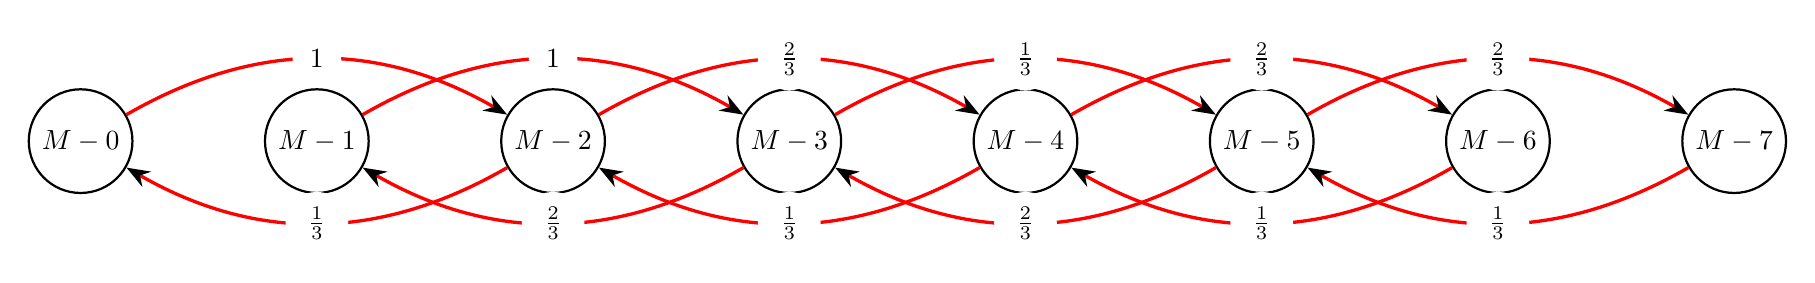
\begin{tikzpicture}
    \begin{scope} [every node/.style={circle,thick,draw}]
        \foreach \i in {7,6,5,4,3,2,1,0}{
            \node (\i) at (3*\i,0) {$M-\i$};
        }
    \end{scope}

    \begin{scope}[>={Stealth[black]},
            every node/.style={fill=white,circle},
            every edge/.style={draw=red,very thick}]
        \path [->] (0) edge[bend left=30] node {$1$} (2);
        \path [->] (1) edge[bend left=30] node {$1$} (3);
        \path [->] (2) edge[bend left=30] node {$\frac{1}{3}$} (0);
        \path [->] (2) edge[bend left=30] node {$\frac{2}{3}$} (4);
        \path [->] (3) edge[bend left=30] node {$\frac{2}{3}$} (1);
        \path [->] (3) edge[bend left=30] node {$\frac{1}{3}$} (5);
        \path [->] (4) edge[bend left=30] node {$\frac{1}{3}$} (2);
        \path [->] (4) edge[bend left=30] node {$\frac{2}{3}$} (6);
        \path [->] (5) edge[bend left=30] node {$\frac{2}{3}$} (3);
        \path [->] (5) edge[bend left=30] node {$\frac{2}{3}$} (7);
        \path [->] (6) edge[bend left=30] node {$\frac{1}{3}$} (4);
        \path [->] (7) edge[bend left=30] node {$\frac{1}{3}$} (5);
    \end{scope}
\end{tikzpicture}

Note that this is only a possible realisation of this chain. It's different if
$M$ is even or odd.

\subsection{b and c and d}
$0 \leftrightarrow 1$ is a transient aperiodic class since you can leave this
class but never come back. It is aperiodic since we can get to state $1$ as
either 2 or 3; $0 \to 0 \to 1$ or $0 \to 1$.
All nodes in this set can communicate thus it is a class.

Of the remaining ones, the evens and odds make up two separate closed,
recurrent, aperiodic communicating classes. They are closed since there is no
way to get to any of the other classes from them.
Since it's a closed finite class then we know they are recurrent.
They are aperiodic because state $2$ and state $3$ can be reached in a single
step.

In the even family we are able to jump from a state to itself, specifically
state $2$. Because of this we have a period of 1 thus it's aperiodic.
It is the same in the odd case since state $3$ has this property.
From these observations we can conclude both these states are aperiodic.

Note that if $M=2$ or $M=3$ then state $2$ and $3$ would be absorbing classes.

\subsection{e}
We make use of local balance equations.
\begin{align*}
    \pi_x p_{xy} &= \pi_y p_{yx}
\end{align*}

We first consider the even communicating class.
\begin{align*}
    \pi_2 p_{2 \to 4} &= \pi_4 p_{4 \to 2} \\
    \pi_2 \frac{1}{3} &= \pi_4 \frac{2}{3} \\
    \pi_2 &= 2 \pi_4 \\
\end{align*}

Since all evens going to another even share the same transition probability
(excluding the $M$ boundary),
we can continue this generally.
\begin{align*}
    \pi_{x-2} &= 2 \pi_x \\
    {\left(\frac{1}{2}\right)}^2 \pi_{x-4} &= \pi_x \\
    {\left(\frac{1}{2}\right)}^3 \pi_{x-6} &= \pi_x \\
    &\vdots \\
    {\left(\frac{1}{2}\right)}^{\frac{x-2}{2}} \pi_{2} &= \pi_x \\
    {\left(\frac{1}{2}\right)}^{i-1} \pi_{2} &= \pi_{2i} \\
\end{align*}

This is true up until the $M$ or $M-1$ term. From here we have a different
probability. Let $2K$ be the upper boundary for the evens regardless of whether
its $M$ or $M-1$.
\begin{align*}
    \pi_{2K-2} p_{(2(K-1) \to 2K)} &= \pi_{2K} p_{(2K \to 2(K-1))} \\
    \pi_{2(K-1)} \frac{1}{3} &= \pi_{2K} 1 \\
    \pi_{2(K-2)} \frac{1}{2} \frac{1}{3} &= \pi_{2K} \\
    &\vdots \\
    \pi_2 {\left(\frac{1}{2}\right)}^{K-2} \frac{1}{3} &= \pi_{2K} \\
\end{align*}

Now we recall that the distributions should sum to 1.
\begin{align*}
    \sum_{i=1}^{\lfloor \frac{M}{2} \rfloor} \pi_{2i} &= 1 \\
    \pi_{M or M-1} + \sum_{i=1}^{\lfloor \frac{M}{2} \rfloor - 1} \pi_{2i} &= 1 \\
    \pi_{M or M-1} + \pi_{2} \sum_{i=1}^{\lfloor \frac{M}{2} \rfloor - 1}
    {\left(\frac{1}{2}\right)}^{i-1} &= 1 \\
    \pi_{M or M-1} + \pi_2
    {\left(\frac{1-\frac{1}{2}^{\lfloor M/2 \rfloor - 1}}{1 - \frac{1}{2}}\right)}
    &= 1 \\
    \pi_2 {\left(\frac{1}{2}\right)}^{\lfloor M/2 \rfloor - 2} \frac{1}{3}
    + \pi_2 {\left(\frac{1-\frac{1}{2}^{\lfloor M/2 \rfloor - 1}}
    {\frac{1}{2}}\right)}
    &= 1 \\
    \pi_2 \left({\left(\frac{1}{2}\right)}^{\lfloor M/2 \rfloor - 2} \frac{1}{3}
    + {\left(\frac{1-\frac{1}{2}^{\lfloor M/2 \rfloor - 1}}{\frac{1}{2}}\right)}\right)
    &= 1 \\
    \pi_2 \left({\left(\frac{1}{2}\right)}^{\lfloor M/2 \rfloor - 2} \frac{1}{3}
    + 2\left(1-\frac{1}{2}^{\lfloor M/2 \rfloor - 1}\right)\right)
    &= 1 \\
    \pi_2 \left({\left(\frac{1}{2}\right)}^{\lfloor M/2 \rfloor - 2} \frac{1}{3}
    + 2 - \frac{1}{2}^{\lfloor M/2 \rfloor - 2}\right)
    &= 1 \\
    \pi_2
    \left({2 - \left(\frac{1}{2}\right)}^{\lfloor M/2 \rfloor - 2} \frac{2}{3} \right)
    &= 1 \\
    \pi_2 \left(2 - \frac{1}{3}{\left(\frac{1}{2}\right)}^{\lfloor M/2 \rfloor - 3}
    \right)
    &= 1 \\
    \pi_2 \left(2 - \frac{1}{3 \times 2^{\lfloor M/2 \rfloor - 3}}\right)
    &= 1 \\
    \pi_2 \left(\frac{2\left(3 \times 2^{\lfloor M/2 \rfloor - 3}\right)-1}{3 \times 2^{\lfloor M/2 \rfloor - 3}}\right)
    &= 1 \\
    \pi_2 \left(\frac{3 \times 2^{\lfloor M/2 \rfloor - 2}-1}{3 \times 2^{\lfloor M/2 \rfloor - 3}}\right)
    &= 1 \\
    \pi_2
    &= \left(\frac{3 \times 2^{\lfloor M/2 \rfloor - 3}}
    {3 \times 2^{\lfloor M/2 \rfloor - 2}-1}\right) \\
\end{align*}

Now that we know $\pi_2$ and have equations for each $\pi_{2i}$ in terms of
$\pi_2$ the limiting distribution for the even class can be found.

We repeat this process for the odds.
\begin{align*}
    \pi_3 p_{3 \to 5} &= \pi_5 p_{5 \to 3} \\
    \pi_3 \frac{2}{3} &= \pi_5 \frac{1}{3} \\
    2 \pi_3 &= \pi_5 \\
\end{align*}

Since all odds going to another odd share the same transition probability
(excluding the $M$ boundary),
we can continue this generally.
\begin{align*}
    2 \pi_{x-2} &= \pi_x \\
    2^2 \pi_{x-4} &= \pi_x \\
    2^3 \pi_{x-6} &= \pi_x \\
    &\vdots \\
    2^{\frac{x-3}{2}} \pi_{3} &= \pi_x \\
    2^{\frac{2i-2}{2}} \pi_{3} &= \pi_{2i+1} \\
    2^{i-1} \pi_{3} &= \pi_{2i+1} \\
\end{align*}

This is true up until the $M$ or $M-1$ term. From here we have a different
probability. Let $2I+1$ be the upper boundary for the odds regardless of whether
its $M$ or $M-1$. Note how this is different to $K$.
\begin{align*}
    \pi_{2(I-1)+1} p_{(2(I-1)+1 \to 2I+1)} &= \pi_{2I+1} p_{(2I+1 \to 2(I-1)+1)} \\
    \pi_{2(I-1)+1} \frac{2}{3} &= \pi_{2I+1} 1 \\
    \pi_{2(I-2)+1} 2 \frac{2}{3} &= \pi_{2I+1} \\
    \pi_{2(I-2)+1} 2^2 \frac{1}{3} &= \pi_{2I+1} \\
    &\vdots \\
    \pi_3 2^{I-1} \frac{1}{3} &= \pi_{2I+1} \\
\end{align*}

Now we recall that the distributions should sum to 1.
\begin{align*}
    \sum_{i=1}^{\lfloor \frac{M}{2} \rfloor} \pi_{2i+1} &= 1 \\
    \pi_{M or M-1} + \sum_{i=1}^{\lfloor \frac{M}{2} \rfloor - 1} \pi_{2i+1} &= 1 \\
    \pi_{M or M-1} + \pi_{3} \sum_{i=1}^{\lfloor \frac{M}{2} \rfloor - 1} 2^{i-1} &= 1 \\
    \pi_3 2^{\lfloor M/2 \rfloor - 1} \frac{1}{3}
    + 2 \pi_{3} \left(\frac{1-2^{\lfloor M/2 \rfloor - 1}}{1-2}\right) &= 1 \\
    \pi_3 2^{\lfloor M/2 \rfloor - 1} \frac{1}{3}
    - 2 \pi_{3} \left(1-2^{\lfloor M/2 \rfloor - 1}\right) &= 1 \\
    \pi_3 \left( 2^{\lfloor M/2 \rfloor - 1} \frac{1}{3}
    - 2 \left(1-2^{\lfloor M/2 \rfloor - 1}\right)\right) &= 1 \\
    \pi_3 \left(\frac{\left(2^{\lfloor M/2 \rfloor - 1}\right)}{3}
    - 2 + 2\times2^{\lfloor M/2 \rfloor - 1}\right) &= 1 \\
    \pi_3 \left(\frac{7}{3} 2^{\lfloor M/2 \rfloor - 1} - 2\right) &= 1 \\
    \pi_3 \left(\frac{7\times2^{\lfloor M/2 \rfloor - 1} - 6}{3}\right) &= 1 \\
    \pi_3 &= \frac{3}{7\times2^{\lfloor M/2 \rfloor - 1} - 6} \\
\end{align*}

\subsection{f}
Because drawing an arbitrary sized row vector is hard we will simply show each
element of this matrix.
There are two limiting distributions for this system. We start at state $0$
which is part of the transitive communicating class. From this class we either
end up in what we will call the evens communicating class or we end up in the
odds communicating class.

The evens communicating class consists of all even numbered states excluding
$0$ and up to $M$.
Likewise, the odds communicating class consists of all odd numbered states
excluding $1$ and up to $M$.

We know our initial state is transitive thus it's guaranteed to leave this
class. We can use this information to determine if we end up in the
evens or odds communicating classes.
\begin{align*}
    \prob(\text{end up in evens} | \text{we leave initial class})
    &= \frac{\prob(\text{end up in evens and we leave initial class})}{\prob(\text{we leave initial})} \\
    &= \frac{\prob(\text{end up in evens})}{\prob(\text{we leave initial})} \\
    &= \frac{^1/_6}{^1/_6 + ^1/_3} \\
    &= \frac{^1/_6}{^1/_2} \\
    &= \frac{1}{3} \\
\end{align*}

\begin{align*}
    \prob(\text{end up in odds} | \text{we leave initial class})
    &= \frac{\prob(\text{end up in odds and we leave initial class})}{\prob(\text{we leave initial})} \\
    &= \frac{\prob(\text{end up in odds})}{\prob(\text{we leave initial})} \\
    &= \frac{^1/_3}{^1/_6 + ^1/_3} \\
    &= \frac{^1/_3}{^1/_2} \\
    &= \frac{2}{3} \\
\end{align*}

From the previous question we know the distributions for both the evens
space and the odds space. For the evens (excluding $0$ and $M$ and $M-1$),
\begin{align*}
    {\left(\frac{1}{2}\right)}^{i-1} \pi_{2} &= \pi_{2i} \\
    {\left(\frac{1}{2}\right)}^{i-1}
    \left(\frac{3 \times 2^{\lfloor M/2 \rfloor - 3}}
    {3 \times 2^{\lfloor M/2 \rfloor - 2}-1}\right)
    &= \pi_{2i}
\end{align*}

Then for $M$ (or $M-1$ whichever is even)
\begin{align*}
    \pi_2 {\left(\frac{1}{2}\right)}^{\lfloor M/2 \rfloor-2} \frac{1}{3} &= \pi_{M\text{ or }M-1} \\
    \left(\frac{3 \times 2^{\lfloor M/2 \rfloor - 3}}
    {3 \times 2^{\lfloor M/2 \rfloor - 2}-1}\right)
    {\left(\frac{1}{2}\right)}^{\lfloor M/2 \rfloor-2} \frac{1}{3} &= \pi_{M\text{ or }M-1} \\
    \left(\frac{2^{\lfloor M/2 \rfloor - 3}}
    {3 \times 2^{\lfloor M/2 \rfloor - 2}-1}\right)
    {\left(\frac{1}{2}\right)}^{\lfloor M/2 \rfloor-2} &= \pi_{M\text{ or }M-1} \\
    \left(\frac{1}{3 \times 2^{\lfloor M/2 \rfloor - 2}-1}\right)
    {\left(\frac{1}{2}\right)} &= \pi_{M\text{ or }M-1} \\
\end{align*}

For the odds (excluding $1$ and $M$ and $M-1$),
\begin{align*}
    2^{i-1} \pi_{3} &= \pi_{2i+1} \\
    2^{i-1} \frac{3}{7\times2^{\lfloor M/2 \rfloor - 1} - 6} &= \pi_{2i+1} \\
\end{align*}

Then for $M$ (or $M-1$ whichever is odd)
\begin{align*}
    \pi_3 2^{\lfloor M/2 \rfloor-1} \frac{1}{3} &= \pi_{M\text{ or }M-1} \\
    \frac{3}{7\times2^{\lfloor M/2 \rfloor - 1} - 6} 2^{\lfloor M/2 \rfloor-1} \frac{1}{3} &= \pi_{M\text{ or }M-1} \\
    \frac{1}{7\times2^{\lfloor M/2 \rfloor - 1} - 6} 2^{\lfloor M/2 \rfloor-1} &= \pi_{M\text{ or }M-1} \\
\end{align*}

The state $1$ will have 0 since it's a transitive state.

\subsection{h}
For the $M \to \infty$ case we don't have an upper bound.
The definition of positive recurrent is that the expected time to return to a
state should be finite. If the expected time is infinite then it is null
recurrent, this should apply for all states in the communicating class.

In the evens case we have a bias towrds the lower bound of state $2$. Because
of this bias we have a non-infinite expectation of returning to state $2$.
The evens communicating class is positive recurrent.

On the other hand, the odds case has a bias towards infinity, it's not likely
that we return to a state ever again. Because of this odds are null-recurrent.

\subsection{i}
In the previous case of using local balance we had to consider the upper bound.
When we don't have an upper bound our equations become much easier.
We first consider the even communicating class.
\begin{align*}
    \pi_2 p_{2 \to 4} &= \pi_4 p_{4 \to 2} \\
    \pi_2 \frac{1}{3} &= \pi_4 \frac{2}{3} \\
    \pi_2 &= 2 \pi_4 \\
\end{align*}

Since all evens going to another even share the same transition probability
we can continue this generally.
\begin{align*}
    \pi_{x-2} &= 2 \pi_x \\
    {\left(\frac{1}{2}\right)}^2 \pi_{x-4} &= \pi_x \\
    {\left(\frac{1}{2}\right)}^3 \pi_{x-6} &= \pi_x \\
    &\vdots \\
    {\left(\frac{1}{2}\right)}^{\frac{x-2}{2}} \pi_{2} &= \pi_x \\
    {\left(\frac{1}{2}\right)}^{i-1} \pi_{2} &= \pi_{2i} \\
\end{align*}

Now recall that the distributions must sum to 1.
\begin{align*}
    \sum_{i=1}^{\infty} \pi_{2i} &= 1 \\
    \pi_{2} \sum_{i=1}^{\infty} {\left(\frac{1}{2}\right)}^{i-1} &= 1 \\
    \pi_{2} \frac{1}{1-{}^1/_2} &= 1 \\
    \pi_{2} &= \frac{1}{2} \\
\end{align*}

For all even states we have,
\begin{align*}
    {\left(\frac{1}{2}\right)}^{i-1} \pi_{2} &= \pi_{2i} \\
    {\left(\frac{1}{2}\right)}^{i-1} \frac{1}{2} &= \pi_{2i} \\
    {\left(\frac{1}{2}\right)}^{i} &= \pi_{2i} \\
\end{align*}

For the odd states we cannot do this. This is because we are making use of the
infinite sum of a geometric sequence.
\begin{align*}
    2 \pi_{x-2} &= \pi_x \\
    2^2 \pi_{x-4} &= \pi_x \\
    2^3 \pi_{x-6} &= \pi_x \\
    &\vdots \\
    2^{\frac{x-3}{2}} \pi_{3} &= \pi_x \\
    2^{\frac{2i-2}{2}} \pi_{3} &= \pi_{2i+1} \\
    2^{i-1} \pi_{3} &= \pi_{2i+1} \\
\end{align*}

\begin{align*}
    \sum_{i=1}^{\infty} \pi_{2i+1} &= 1 \\
    \pi_{3} \sum_{i=1}^{\infty} {\left(2\right)}^{i-1} &= 1 \\
\end{align*}

We cannot add an infinite sum of these terms. Therefore the only solution
is to set $\pi_{3} = 0$ and by extension $\pi_{2i+1} = 0, \forall i \in \mathbb{N}$.

\section{4}
\subsection{a}
For the move to be accepted we must first generate the move from the easier,
proposal distribution. From this we then weigh up if this proposed move gets
accepted. This will happen if it passes the acceptance probability.

We must first observe the relationship between $\alpha_{xy}$ and $\alpha_{yx}$.
Suppose $\frac{p_y q_{yx}}{p_x q_{xy}} > 1$. Then,
\begin{align*}
    \frac{p_y q_{yx}}{p_x q_{xy}} &> 1 \\
    1 &> \frac{p_x q_{xy}}{p_y q_{yx}} \\
    1 &> \alpha_{yx} \\
\end{align*}

Thus if $\alpha_{xy} = 1$ then $\alpha_{yx} \leq 1$.

Without loss of generality let $\alpha_{yx} = 1$.
The local balance equation is as follows,
\begin{align*}
    \pi_{X} p_{X \to Y} &= \pi_{Y} p_{Y \to X} \\
    \pi_{X} q_{xy} \alpha_{xy} &= \pi_{Y} q_{yx} \alpha_{yx} \\
    \pi_{X} q_{xy} \frac{p_y q_{yx}}{p_x q_{xy}} &= \pi_{Y} q_{yx} \\
    \pi_{X} p_y &= \pi_{Y} p_{x} \\
\end{align*}

Thus our acceptance probability still allows us to approach the same
limiting distribution as our target distribution.

\end{document}
